\documentclass[10pt,a4paper]{article}
\usepackage{amsmath}
\usepackage[utf8]{vietnam}
\usepackage{amsfonts}
\usepackage{amssymb}
\usepackage{graphicx}
\usepackage[left=2cm,right=2cm,top=2cm,bottom=2cm]{geometry}
\setlength{\parindent}{0pt}

\begin{document}

\begin{center}
    \fontsize{30}{30}\selectfont
    PHƯƠNG PHÁP THIẾT KẾ
\end{center}
\begin{flushleft}
\fontsize{14}{20}\selectfont
\part{Cách tiếp cận bài toán}
Thay vì tính số món hàng lớn nhất có thể mua được với c đồng, ta sẽ tính số  tiền nhỏ nhất để mua j món đồ cho mọi j có thể (j bé hơn hoặc bằng n), sau đó ta tìm j lớn nhất sao cho số tiền mua j món đó không vượt quá c đồng.\\
\vspace{0.5 cm}
Có thể thấy dữ liệu của bài toán này có thể quy về dạng cây:\\
\hspace{1 cm}- Gốc là node 1 hay đại diện cho món đồ đầu tiên.\\
\hspace{1 cm}- Mỗi node đại diện cho một món đồ, hai node là kề nhau nếu thỏa điều kiện: muốn dùng phiếu giảm giá cho món đồ thứ i phải dùng phiếu giảm giá cho món đồ thứ $x_i$, khi đó node $x_i$ là cha, node i là con. Ví dụ muốn dùng phiếu giảm giá cho món đồ thứ 3 thì phải dùng phiếu giảm giá cho món đồ thứ 2: khi đó node 2 là cha, node 3 là con.\\
\hspace{1 cm}- Điều kiện $x_i$ < i đảm bảo không có chu trình trong cây.\\
\hspace{1 cm}- Ràng buộc về phiếu giảm giá(tức là dùng phiếu giảm giá cho món đồ thứ $x_i$ trước khi dùng phiếu giảm giá cho món đồ thứ i) về bản chất là nếu mua món đồ thứ i với giá đã được giảm, thì ta phải mua món đồ thứ $x_i$ với giá đã được giảm.\\
\vspace{0.5 cm}
Vì vậy, chúng ta sẽ sử dụng phương pháp quy hoạch động trên cây để giải quyết bài toán này.\\
\hspace{1 cm}- Gọi F[i][j] là chi phí tối thiểu để mua được j món hàng trong cây con của node cha i có thể dùng phiếu giảm giá.\\
\hspace{1 cm}- G[i][j] là chi phí tối thiểu để mua được j món hàng trong cây con của node cha i mà không dùng phiếu giảm giá.\\
\vspace{0.5 cm}
Bài toán có ba bước chính:\\
\hspace{1 cm}- Ta dùng duyệt sâu (DFS) để duyệt đến các node của cây.\\
\hspace{1 cm}- Ta thực hiện tính F[i][j] và G[i][j] cho từng node i thuộc cây.\\
\hspace{1 cm}- Tìm j món đồ lớn nhất sao cho giá của nó không vượt quá c đồng.\\
\part{Cách hiện thực bài toán}
Đầu tiên, chúng ta cần khởi tạo các mảng gồm:\\
\hspace{1 cm}- Mảng 1 chiều a, với a[i] là số tiền mua món đồ thứ i mà không dùng phiếu giảm giá.\\
\hspace{1 cm}- Mảng 1 chiều b, với b[i] là số tiền có thể giảm khi mua món đồ i mà có dùng phiếu giảm giá.\\
\hspace{1 cm}- Mảng gg[][] là mảng hai chiều để lưu cây dưới dạng danh sách kề.\\
\hspace{1 cm}- Mảng 2 chiều F, với F[i][j] là  chi phí tối thiểu để mua được j món hàng trong cây con có đỉnh i là gốc có thể dùng phiếu giảm giá.\\
\hspace{1 cm}- Mảng 2 chiều G, với G[i][j] là chi phí tối thiểu để mua được j món hàng trong cây con có đỉnh i là gốc mà không dùng phiếu giảm giá.\\
\hspace{1 cm}- Mảng 1 chiều sz, với sz[i] là số lượng đỉnh đã duyệt thuộc cây con có đỉnh i là gốc.\\
\vspace{0.5 cm}
Sử dụng phương pháp duyệt sâu để tính toán các giá trị của cây từ node lá ngược lên node gốc.\\
\vspace{0.5 cm}
Có thể thấy rằng nếu node i là lá thì:\\
\hspace{1 cm}- F[i][j]=a[i]-b[i] vì i không có con.\\
\hspace{1 cm}- G[i][j]=a[i] tương tự như trên.\\
\hspace{1 cm}- sz[i]=1 vì node lá chỉ có mình nó.\\
Để tính F[i][j] và G[i][j] cho các node không phải lá:\\
\hspace{1 cm}- Ban đầu chúng ta xem nó như node lá, tức là không có cây con thuộc nó và giá trị khởi tạo ban đầu gồm:\\
\hspace{2 cm} F[i][1]=a[i]-b[i]\\
\hspace{2 cm} G[i][0]=0\\
\hspace{2 cm} G[i][1]=b[i]\\
\hspace{2 cm} sz[i]=1\\
\hspace{1 cm}- Sau đó, chúng ta cần duyệt sâu để tính các giá trị mảng F, G cho các node con của i trước, và lần lượt thêm các cây con đó vào node cha i, tiến hành cập nhật mảng F[i][j], G[i][j] và sz[i] cho node cha i sau mỗi lần thêm cây con vào:\\
\hspace{2 cm} Cho j chạy từ sz[i] ngược về 0 và k chạy từ 0 đến sz[v] với v là con của i, ta tiến hành cập nhật như sau:\\
\hspace{3 cm} G[i][j+k]=min(G[i][j+k], G[i][j]+G[v][k])\\
\hspace{3 cm} F[i][j+k]=min(F[i][j+k],F[i][j]+min(g[v][k],f[v][k]))\\
\hspace{2 cm} sz[i]+= sz[v]\\
\vspace{0.5 cm}
Sau khi tính được mảng F và G, ta sẽ tìm giá trị j lớn nhất sao cho F[1][j] bé hơn hoặc bằng c hoặc G[1][j] bé hơn hoặc bằng c hay nói cách khác là mua nhiều món đồ nhất thuộc node 1(node gốc, có kích thước sz[1] = n tương đương với tìm nhiều món đồ nhất trong n món đồ) sao cho giá tiền của j món đồ đó không vượt quá c, đó chính là kết quả của bài toán.
\end{flushleft}
\fontsize{14}{20}\selectfont
\bfseries 
Ví dụ minh họa\\
\mdseries
Input:
6 16\\
10 9\\
10 5 1\\
12 2 1\\
20 18 3\\
10 2 3\\
2 1 5\\
\begin{center}
     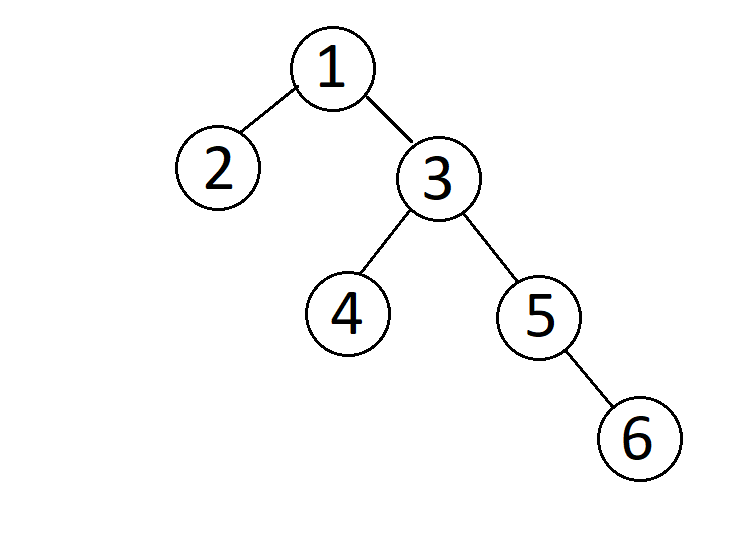
\includegraphics[scale=.5]{vidu.png} \\
\end{center}

\end{document}